\documentclass[12pt]{article}
\usepackage{amsmath}
\usepackage{graphicx}
\usepackage{amssymb}
\usepackage{mathtools}
\usepackage{color}

\graphicspath{ {D:/Bilder/Latex/} }

\title{Set Theory cheat sheet}
\author{Hampus Weslien}
\date{\today}



\begin{document}
\maketitle
\clearpage


\section{Sets}
\begin{description}
\item[Cardinality:] Cardinality is the number of elements in a set A, written $\#(A)$ or $\left|A\right|$. Useful formula for the number of combinations: $\frac{n!}{k!(n-k)!}$

\item[Difference] Difference, $x \in A\backslash B$ iff $x \in A$ or $x \in B$

\item[Disjointness] Two sets A and B are disjoint if they do not have any common elements: $A \cap B = \emptyset$

\item[Inclusion:] Inclusion refers to $A\subseteq B$, this means that if $x \in A$ then $x \in B$

\item[Intersection] Intersection, $x \in A \cap B$ iff $x \in A$ or $x \in B$

\item[Poset (partially ordered set):] A poset $(A,<)$ is well-founded iff all non-empty subsets $X \subseteq A$ have a minimal element, i.e.  for some $m \in X$ and all $a \in X, a \not< m$

\item[Power set] The power set of a set A is the set of all its subsets, \\ $P(A) = \{s: s \subseteq A \} = 2^A$ 

\item[Union:] The union, $x \in A \cup B$ iff $x \in A$ or $x \in B$
\end{description}


\subsection{Syntax}
\begin{description}
\item[Generalized union and intersection:]
\begin {math} \\
\bigcup S = \{x: x \in s \textrm{ for at least one } s \in S \} \\
\bigcap S = \{x: x \in s \textrm{ for all } s \in S \} \\ \\
\textbf{Example:}\\ \begin{array}{ccc} 
\bigcup\{A_i : i \in I\} & \bigcup\{A_i\}_{i \in I} & \bigcup_{i \in I}  A_i \\
\bigcap\{A_i : i \in I\} & \bigcap\{A_i\}_{i \in I} & \bigcap_{i \in I}  A_i 
\end{array}
\end {math} 

\item[List comprehension]: \\ \begin {math} \begin{array}{cc} 
\textrm{flavor 1} & \textrm{flavor 2} \\
\{ n \in \mathbb{N}^{+} : n \textrm{ is prime} \} & \{ n: n \in \mathbb{N}^{+} , n \textrm{ is prime} \} \\
\{ n \in \mathbb{N}^{+} \| n \textrm{ is prime} \} & \{2n: n \in \mathbb{N}^{+} \} 
\end{array}
\end {math} \\

\item[Families of sets] 
\begin {math} \\
\{ N_i : i \in \mathbb{N} \} \textrm{ with } N_i = \{ k \in \mathbb{N} : k \geq i\}
\end {math}
\end{description}


\section{Relations}

\begin{description}
\item[Antisymmetry:] A binary relation $R = A \times A$ is antisymmetric iff for all $a,b \in A $ if $aRb$ and $bRa$ then $a = b$

\item[Asymmetry:] A binary relation $R = A \times A$ is asymmetric iff for all $a,b \in A $ if $aRb$ then not $bRa$

\item[Cartesian product:] The (cartesian) product of a pair of sets, or more generally a finite family of sets, is the set of all ordered pairs or n-tuples. \[A_1 \times ... \times A_n = \{(a_1 , ... , a_n): a_1 \in A_1, ... , a_n \in A_n\}\]

\item[Closure:] Given a relation $R \subseteq A \times A$ and a set $X \subseteq A$, the closure of X under R $R[X]$ is defined as the smallest $Y \subseteq A$ such that $X \subseteq Y$ and $R(Y) \subseteq Y$

\item[Closure of relations, rules, generators:] Given a set $A$, a family of relations on A $R = \{R_i \subseteq A^{n_i}: i \in I\}$ and a set $X \subseteq A$, the closure of X under R $R[X]$ is defined as the smallest $Y \subseteq A$ such that $X \subseteq Y$ and $R_i (Y^{n_i})\subseteq Y$ for all $i \in Y$.

\item[Complement:] For a binary relation $R = A \times B$ its complement is the relation 
\[ \overline{R} = A \times B \textrm{\textbackslash} R\]

\item[Composition:] Given two binary relations $R = A \times B$  and $S = B \times C$ their composition is a binary relation on  $A \times C$ \[ S \circ R = \{(a,c): aRb  \textrm{ and } bSc \textrm{ for some } b \in B\}\]

\item[Converse:] For a binary relation $R = A \times B$ its converse (inverse) is the relation \[ R^{-1} = \{(b,a): aRb\}\]

\item[Equinumerosity principle:] $\#(A) = \#(B)$ iff there is some bijection \\$f: A \to B$

\item[Image:] Given a binary relation $R = A \times B$ from A to B, for any $a \in A$ its image under $R$, written $R(a)$, is defined as $R(a) = \{b \in B : aRb\}$

\item[Irreflexivity:] A binary relation $R = A \times A$ is irreflexive iff there is no $a \in A  \quad aRa$

\item[N-tupels:] $(a_1,...,a_n) = (b_1,...,b_n)$ iff $a_i = b_i$ for $i = 1,...,n$

\item[Order relation, poset:] A binary relation $\preceq \subseteq A \times A$ is an (inclusive or non-strict) (partial) order iff it is
\begin{enumerate}
	\item Reflexive
	\item Antisymmetric
	\item Transitive
	\end{enumerate}	

\item[Ordered pairs, tupels:] $(a,b) = (x,y)$ iff $a = x$ and $b = y$

\item[Partitions:] Given a set A, a partition of A is a set of pairwise disjoint sets
$\{B_i : i \in I \}$, such that \[ A = \bigcup_{i \in I} B_i\]

\item[Reflexivity:] A binary relation $R = A \times A$ is reflexive iff for all $a \in A  \quad aRa$

\item[Similarity relationship:] A similarity relationship had two properties,
	\begin{enumerate}
	\item Reflexive
	\item Symmetric
	\end{enumerate}	 
	
\item[Strict (partial) order] A binary relation $\prec \subseteq A \times A$ is a strict (partial) order iff it is
\begin{enumerate}
	\item Irreflexive
	\item Transitive
	\end{enumerate}		

\item[Symmetric closure:]The symmetric closure $S$ of a relation $R$ on a set $X$ is given by $S = R \cup \{(x,y): (y,x) \in R\}$. In other words, the symmetric closure of $R$ is the union of $R$ with its inverse relation, $R^{-1}$.
	
\item[Symmetry:] A binary relation $R = A \times A$ is symmetric iff for all $a,b \in A $ if $aRb$ then $bRa$	

\item[Total (or linear) order] A binary relation $\preceq \subseteq A \times A$ is a (non-strict) total (or linear) order iff it is
\begin{enumerate}
	\item Irreflexive
	\item Antisymmetric
	\item Transitive
	\item Total (complete): $a \preceq b \textrm{ or } b \preceq a$
	\end{enumerate}	

\item[Transitive clojure:] It's the smallest set R* in which R is a subset and we have added relations to make it transitive.

\item[Transivity:] A binary relation $R = A \times A$ is transitive iff for all $a,b,c \in A$ if $aRb  \wedge bRc \rightarrow aRc$ 
\end{description}


\section{Functions}

\begin{description}

\item[Bijection:] A function $f: A \rightarrow B$ is bijective iff it it is both injective and surjective  Notation: $f: A \longleftrightarrow  B$

\item[Composition:] Given functions $f: A \rightarrow B$ and $g: B \rightarrow C$ their composition $g \circ f: A \rightarrow C$ defines as $g \circ f = g(f(a))$

\item[Closure:] Given an endofunction $f: A \rightarrow A$ and a set $X \subseteq A$, the closure of X under f $f[X]$ is defined as the smallest $Y \subseteq A$ such that $ X \subseteq Y$ and $F(Y) \subseteq Y$


\item[Equivalence relations:] A binary relation $\approx \subseteq A \times A$ is an equivalence relation iff it is
	\begin{enumerate}
	\item Reflexive
	\item Symmetric
	\item Transitive
	\end{enumerate}	

\item[Image:] Given a function $f: A \rightarrow B$ and a set $X \subseteq A$, the image of $X$ under $f$ is defined as $f(X) = \{f(a): a \in X\}$	
	
\item[Injection:] A function $f: A \rightarrow B$ is injective iff $a \neq b$ implies $f(a) \neq f(b)$ Notation: $f: A \xhookrightarrow{} B$

\item[Inverse:] given a function $f: A \rightarrow B$ its inverse (converse) $f^{-1} \subseteq B \times A$ is defined as: $f^{-1} = \{ (F(a),a): a \in A \}$

\item[Restriction of a function:] Given a function $f: A \rightarrow B$, its restriction to a set $X \subseteq A$ is defined as \[ \begin{array}{cc}
f_X : X \rightarrow B & f | X \\
a \mapsto f(a) & \textrm{alternative syntax}
\end{array} \]

\item[Set of all functions:] $B^A \qquad  \langle A \rightarrow B \rangle \qquad \# (B^A) = \#(B)^{\#(A)}$

\item[Surjection:] A function $f: A \rightarrow B$ is surjective iff $f(A = B)$ \\ Notation: $f: A \twoheadrightarrow  B$

\end{description}


\section{Notation}

\begin{description}
\item[Equivalence class:] $[x]$ is the equivalence class containing all elements that are considered equal to x in a some predefined relation.

\item[The set of all functions:] $B^A$ is the set of all functions from set A to set B

\item[Weird naming]: \\
\begin{math} \begin{array}{ccc}
& R \subseteq A \times B & f: A \rightarrow B \\
\textrm{actual values, left} & \textrm{domain} & \textrm{domain}\\
\textrm{actual values, right} & \textrm{range} & \textrm{range} \\
\textrm{A} & \textrm{source} & \textrm{domain} \\
\textrm{B} & \textrm{target} & \textrm{codomain} 
\end{array}
\end{math}

\end{description}

\section{Infinity}
\begin{description}

\item[Cantor-Schröder-Bernstein theorem (CSB):] For ant two sets A and B, if there are two injections $f: A \xhookrightarrow{} B$ and $g: B \xhookrightarrow{} A$ then there exists a bijection $h: B \longleftrightarrow B$ \\
Corollary: if $\# (A) \leq \# (B)$ and $\# (B) \leq \# (A)$ then $\# (A) = \# (B)$ 

\item[Denumerable:] A is denumerable (countable) if it is equinumerous to the natural numbers, i.e. $S \sim \mathbb{N}$ \\ The cardinality of the natural numbers $\#(\mathbb{N}) =  \aleph_0$

\item[Finite sequences/strings:] Let A be a finite set of n symbols $A = \{a_1,...,a_n\}$. The set of all finite sequences (strings) of these symbols is $A^{*}$. The empty sequence is $\epsilon \in A^{*}$

\item[Infinite sequences:] Let A be a finite set of n symbols $A = \{a_1 , ... ,a_n\}$. An infinite sequence in A is a function $s: \mathbb{N} \rightarrow A$. The set of all infinite sequences in A: $A^\mathbb{N}$ 

\item[Infinity:] A is infinite if it is equinumerous to a proper subset of itself. That is, there is some S such that $S \subset A$ and $S \sim A$


\item[Rational numbers:]  \begin{itemize}
\item [1]$\mathbb{Q}$ is dense: between any two distinct $r,s \in \mathbb{Q}$ there is $\frac{r + s}{2} \in \mathbb{Q}$
\item [2]Any non-empty open interval $]r,s[ \subset \mathbb{Q}$ is equinumerous to $ \mathbb{Q}$
\end{itemize}

\end{description}

\textbf{Example:} Bijection between a subset of the real numbers and the real numbers 
\begin{align*}
& p_{\mathbb{R}}: ]0,1[_{\mathbb{R}} \longleftrightarrow \mathbb{R}´\\
& x \longmapsto \Bigg\{ \begin{array}{c}
\frac{1}{x} - 2 \textrm{ for } x < \frac{1}{2} \\
2 - \frac{1}{x - 1} \textrm{ for } x \geq \frac{1}{2} 
\end{array}
\end{align*}

\section{Proofs}

\begin{description}

\item[Contrapositive proof $(\neg C \implies \neg P)$]:
\begin{enumerate}
\item[Theorem:] If $x^2 -6x +5$ is even, then x is odd.

\item[Proof:] Suppose $x$ \textcolor{red}{is even}. There is an integer $a$ such that $x = 2a$.$x^2 -6x +5 = 4a^2 -12a + 4 +1 = 2(2a^2 -6a +2) +1$ So there is an integer b s.t. $x^2 -6x +5 = 2b +1$ Therefore $x^2 -6x +5$ \textcolor{red}{is not even.}

\end{enumerate}


\item[Direct proof]: 
\begin{enumerate}
\item[Theorem:] If $x$ is odd, then $x^2$ is odd

\item[Proof:] Suppose x is odd. Theredore, there is an integer $k$ such that $x = 2k + 1$. Thus $x^2 =(2k + 1)^2= 4k^2 + 4k +1 = 2(2k^2 +2k) +1$. Note that $2k^2 +2k$ is an integer. thus there is an integer n such that $x^2 = 2n+1$. Therefore $x^2$ is odd.

\end{enumerate}

\item[Direct proof with cases]:
\begin{enumerate}
\item[Theorem:] If $n \in \mathbb{N}$ then $1 + (-1)^n(2n-1)$ is a multiple of 4.

\item[Proof:] Suppose $n \in \mathbb{N}$. Then n is either even or odd.

\item[Case 1:] Suppose $n$ is even. Then $n=2k$ for some $k \in \mathbb{Z}$. Thus $1 + (-1)^{2k}(2(2k)-1) = 1 +1^k(4k-1) = 4k$. That is a multiple of 4.

\item[Case 2:] Suppose $n$ is odd.  Then $n=2k +1$ for some $k \in \mathbb{Z}$. Thus $1 + (-1)^{2k +1}(2(2k +1)-1) = 1 -(4k +2 -1) = -4k$. That is also a multiple of 4. 
\end{enumerate}

\item[Proof by contradiction]:
\begin{enumerate}
\item[Theorem:] If $a,b \in \mathbb{Z}$ then $a^2 - 4b \neq 2$

\item[Proof:] Suppose there are $a,b \in \mathbb{Z}$ s.t. $a^2 - 4b = 2$. Sinice this implies $a^2 = 4b +2 = 2(2b + 1), \; a^2$ is even. Hence $a$ is even, so $a = 2c$ for some integer $c$. Thus $4c^2 - 4b = 2$, i.e. $2c^2 -2b = 1$. Therefore $2(c^2 - b) = 1$ with $c^2 -b in \mathbb{Z}$. So 1 is even.

\end{enumerate}
\end{description}

\section{Induction and Recursion}
\begin{description}
\item[Cumulative (complete) induction]:\\ 
\begin{tabular}{l c}
Hypothesis: & $P(n)$  \\
Basis: & $P(0)$  \\
Induction step: & Assuming that $P(m)$ for all $m < k$ show that $P(k)$
\end{tabular}
\item[Simple induction]:\\ 
\begin{tabular}{l c}
Hypothesis: & $P(n)$ for all n \\
Basis: & Show that $P(1)$ (or $P(0)$ or some other, depending on circumstances) \\
Induction step: & Assuming that $P(k)$ show that $P(k + 1)$
\end{tabular}
\item[Structural induction]:\\ 
\begin{tabular}{l c}
Hypothesis: & $P(x)$  for all $x R[X]$ \\
Basis: & $P(x)$ for all $x \in X$  \\
Induction step: & All rules $R_i \in R$ preserve the property: if their ''input'' objects have it, \\ 
& then so does their “output” object. 
\end{tabular}
\item[Structural recursion on domains]:\\ 

\begin{math}  \begin{array}{cc}
 R = \{R_1 ,R_2 ,R_3 \}, \quad C = UTF-16 & R_1 = \{(s,"-" s): s \in C^*\} \\
 V = \{ \textrm{"a" , ... , "z"}\}\setminus \{\epsilon\} & R_2 = \{(s_1,s_2, "(" s_1 "+" s_2 ")"): s_1 , s_2 \in C^*\}
\end{array}
\end{math}

\begin{math}
eval_E : R[V] \rightarrow \mathbb{R} \\
eval_E : s \mapsto  \begin{cases}
 E(s) & \textrm{ for } s \in V \\
 -eval_E (s') & \textrm{ for } s = "-" s' \\
 eval_E (s_1) + eval_E (s_2) & \textrm{ for } s = "(" s_1 "+" s_2 ")" \\
 eval_E (s_1) \dot eval_E (s_2) & \textrm{ for } s = "(" s_1 "*" s_2 ")"
\end{cases}
\end{math} 

 \item[Well-founded induction:] Given a well-founded set $(A,<)$ and a property $P(a), a \in A$, if for all $a in A: P(w)$ for all $w < a$ implies $P(a)$ then $P(a)$ for all $a \in A$
\item[Well-founded recursion:] Given a well-founded set $(W,<)$and a recursive function definition for a function $f:W \rightarrow X$, f is well-defined if it computes the value for every $w \in W$ only depending on values of f for $v < w$.
\end{description}

\section{Trees and Graphs}
\begin{description}
\item[Binary search trees:] Given a labelled binary tree  $(V, R)$, with labelling function $\lambda : T \rightarrow L$ and a
totally ordered label set L. It is a binary search tree iff for all nodes their label
is greater than any label in their left subtree, and less than any label in their
right subtree. 

\item[Binary trees:] Given a tree $(V, R)$ with root a, we say it is binary if every node has at most two children and there is a labeling function
\[\beta : T \backslash \{a\} \rightarrow \{left,right\}\]
such that no two children of the same node are labelled identically.

\item[Cycles:] A cycle is a path $a_0 , ... , a_n$ where $a_0 = a_n$. A graph that does not contain cycles is called acyclic.

\item[Graphs:] A (directed) graph is a pair $(V, E)$ where $V$ is a finite set of vertices (or nodes) and a relation $E subseteq V \times V$, a set of (directed) edges (or arcs).

\item[Labeled trees:] Given a tree $(V, R)$, and a set of labels $L$, a labelling is a function $\lambda : T \rightarrow L$. A tree with a labelling is called a labelled tree

\item[Ordered trees:] Given a tree  $(V, R)$ with root a, we say it is ordered if there is a function \[\mu : T \backslash \{a\} \rightarrow \mathbb{N}^{+}\]
such that for every node its n children are labelled $1 ... n$.


\item[Paths:] Given a graph $(V, E)$, a path is a finite sequence $a_0 , ... , a_n$ in $V$ with $n \geq 1$ such that for .The length of the path is n.

\item[Spanning trees:] Given an undirected graph $(T,S)$, an unrooted tree $(T,R)$ is a spanning tree for it iff $R subseteq S$

\item[Trees:] A (rooted) tree is a graph $(T,R)$ such that T is empty or there is an $a \in T$ such that:
\begin{enumerate}
\item[(i)] for every $x \in T, x \neq a$ there is exactly one path from a to x
\item[(ii)] there is no path from a to a. 
\end{enumerate}
\textbf{Properties: }
\begin{enumerate}
\item[1] Any non-empty tree has a unique root.
\item[2] A root has no parent.
\item[3] Every non-root has exactly one parent.
\item[4] A tree with n nodes has n-1 links
\item[5] A tree contains no cycles.
\end{enumerate}

\item[Undirected graphs:] An (undirected) graph is a pair $(V, E)$ where $V$ is a set of vertices (or nodes) and a
symmetric relation $E subseteq V \times V$, a set of (undirected) edges (or arcs).

\item[Unrooted trees:] A structure $(V, S)$ is an unrooted (undirected)tree iff
 $(V, R)$ is a rooted tree and S is the symmetric closure of R.

\item[Defining trees recursively]: \\
\begin{enumerate}
\item[1] The empty graph $(\emptyset , \emptyset)$ is a tree.
\item[2] Given a family of disjoint trees $(T_i , R_i)_i$ = 1..n, i.e. $T_i \cap T_j = \emptyset$ when $i \neq j$,
 and with roots $B = \{b_i : 1 \leq i \leq n\}$, as well as a fresh $a \notin   \bigcup_{i \in 1..n} R_i$ we can
 create a new tree with root a: 
\end{enumerate}
\end{description}


\section{Propositional Logic}
\begin{description}
\item[Assignments and valuations:] Given a set of elementary letters E and an assignment v, a valuation is the recursive extension of v over the set F[E] of formulae in E generated by a set of rules F: \[v^{+} F[E] \rightarrow  \{1,0\}\]

\item[Tautological implication:] Given a set of formulae A and a formula $\beta$ we say that A
tautologically implies $\beta$ if there is no valuation v such that \[v(\alpha) = 1 \textrm{ for all } \alpha \in A \textrm{ and } v(\beta) = 0\] \[A \models B \qquad A \vdash B\]

\item[Tautological equivalence:] Given two formulae $\alpha$ and $\beta$, we say that they are tautologically equivalent if they tautologically imply each other.\[\alpha \dashv \: \vdash \beta\]

\end{description}

\begin{figure}[htbp]
\hspace{-2cm}    
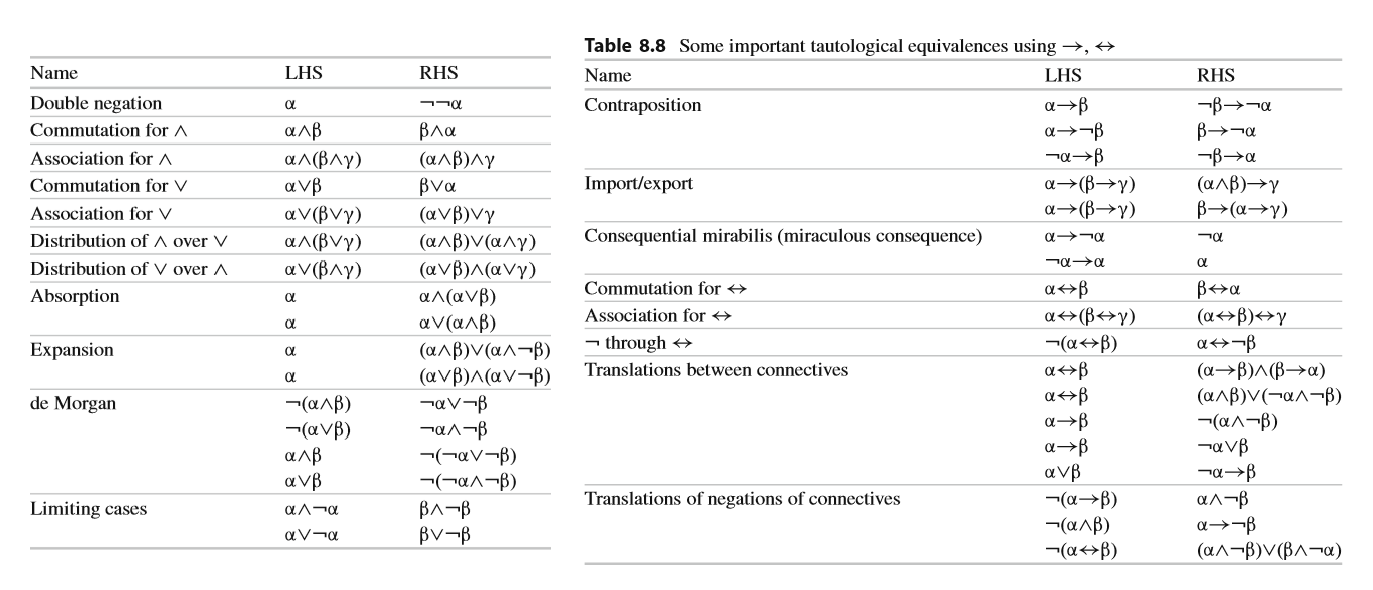
\includegraphics[scale=.5]{tabell3}
\end{figure}

\section{Quantificational Logic}

\begin{description}
\item[Free and bound variable occurrences: ] A variable occurrence is bound iff it occurs inside the scope of a quantifier
that binds that variable. It is free otherwise. \\ \\
A formula with no free variable occurrences is called closed.
A closed formula is a sentence.

\item[Logic with quantifiers (informally):] logic with quantifiers (informally)
\begin{enumerate}
\item[] $\forall x(\alpha)$ represents “forall x, $\alpha$“ alt. notation $\underset{x}{\wedge} \alpha$
\item[] $\exists x(\alpha)$ represents “there exists an x, such that $\alpha$” alt. notation $\underset{x}{\vee}\alpha$
\end{enumerate}

\item[Quantifier scopes:]


\end{description}
\begin{figure}[h]
\centering 
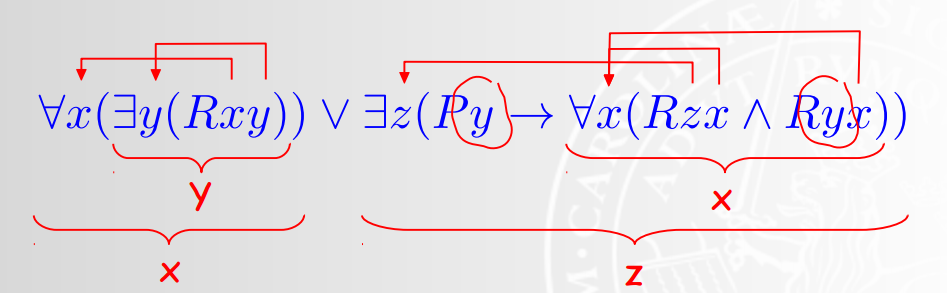
\includegraphics[scale=.5]{scope}
\end{figure}
\end{document}

